% !TeX root = RJwrapper.tex

\title{\pkg{rotations}: A Package for $SO(3)$ Data}
\author{by Bryan Stanfill, Heike Hofmann, Ulrike Genschel}

\maketitle

\abstract{
In this article we introduce the \pkg{rotations} package which provides users with the ability to simulate, analyze and visualize three-dimensional rotation data.  The \pkg{rotations} package gives the user access to four distributions from which to simulate data, four estimators of the central orientation, three confidence region estimation procedures and a novel approach to visualizing these data.  All of the above features are available to two different parameterizations of rotations: three-by-three matrix form and quaternions.
}

\section{Introduction}

Data in form of three-dimensional rotations find application in several scientific areas, such as bio-medical engineering, computer visioning, and geological and materials sciences where such data represent the positions of objects within some three-dimensional reference frame.  For example, \cite{humbert1996, bingham2009, bachmann2010} use rotation data to study the orientation of crystals on metal surfaces.  \cite{rancourt2000} use this data to represent an individual's body position whilst performing a task. 

A common goal shared by these fields is to estimate the main or central orientation for a sample of rotations.  That is, letting the rotation group $SO(3)$ denote the collection of all $3\times 3$ rotation matrices, observations $\bm{R}_1,\ldots,\bm{R}_n \in SO(3)$ can be conceptualized as a random sample from a \textit{location model}
\begin{equation}
\label{eqn:loc_model}
\mathbf{R}_i = \bm{S} \bm{E}_i, \quad i=1,\ldots,n,
\end{equation}
where $\bm S \in SO(3)$ is the {\it fixed} parameter of interest indicating an orientation of central tendency, and $\bm{E}_1,\ldots,\bm{E}_n \in SO(3)$ denote i.i.d. {\it random} rotations which symmetrically perturb $\bm{S}$.  The data-generating model in \eqref{eqn:loc_model} is a rotation-matrix analog of a location model for scalar data $Y_i = \mu + e_i$, where $\mu \in \mathbb{R}$ denotes a mean and $e_i \in \mathbb{R}$ denotes an additive error symmetrically distributed around zero.

For the scaler location model a multitude of methods for location models are available in R, but for the case of $SO(3)$ data the toolbox is more limited.  The \CRANpkg{orientlib} package includes the definition of an orientation class along with a few methods to summarize and visualize rotation data \citep{murdoch2003}.  A strength of the \CRANpkg{orientlib} package is its thorough exploration of rotation representations, but no methods for inference are available and the estimation and visualization techniques are lacking.  The \pkg{uarsbayes} package includes functions for data generation and Bayes inference but is not publicly available \citet{qu2013}.  In addition there are several packages for circular and spherical, e.g. \CRANpkg{circular}, \CRANpkg{SpherWave}, data but their extension to rotation data is non-trivial.

The \pkg{rotations} package provides users with the tools necessary to simulate rotations from \eqref{eqn:loc_model} with several distributional models for the perturbation matrices $\bm E_i$.  Estimation and inference for $\bm{S}$ in \eqref{eqn:loc_model} is also available along with novel visualization techniques.  The remainder of this manuscript introduces rotation data more fully and discusses the ways they are handled by the \pkg{rotations} package.


\section{Rotation Parameterizations}

Several parameterizations of rotations exist, we consider two of the most popular: matrices in $SO(3)$ and four-dimensional unit vectors called \dfn{quaternions}.  

\subsection{Matrix Form}

Rotations in three-dimensions can be represented by $3\times3$ orthogonal matrices with determinant one.  Matrices with these characteristics form a group called the \dfn{special orthogonal group}, or \dfn{rotation group}, denoted $SO(3)$.  Every element in $SO(3)$ can be described by an angle, $r\in[0,\pi)$ and an axis, $\bm u\in\mathbb{R}^3$ with $\|\bm u\|=1$, which in the material scientist's literature are called the \dfn{misorientation angle} and the \dfn{misorientation axis}, respectively.  

More specifically, given an angle $r$ and axis $\bm u=(u_1,u_2,u_3)$ the rotation matrix $\bm R\in SO(3)$ is formed by
\begin{equation}\label{eqn:angleaxis}
 \bm{R} = \bm{R}(r,\bm{u}) = \bm{u}\bm{u}^\top+(\bm{I}_{3\times3}-\bm{u}\bm{u}^\top)\cos(r) +\Phi(\bm{u})\sin(r)
\end{equation}
where
\[
\Phi(\bm{u}) = \Phi (u_1,u_2,u_3) = \left(\begin{array}{ccc}0 & -u_3 & u_2 \\ u_3 & 0 & -u_1 \\-u_2 & u_1 & 0\end{array}\right).
\]
For more details on this construction see Stanfill et al. (2013) (or some other reference).

The function \code{SO3} creates a rotation matrix according to \eqref{eqn:angleaxis} for a variety of inputs.  Given an angle and axis \code{SO3} will form a matrix as described above; given only a three-dimensional vector the length of that vector will be taken to be the angle of rotation and the vector will be made unit length.  One can also supply a rotation in the quaternion representation and the matrix equivalent will be return as an \code{SO3} object.  A rotation matrix is returned in vector form with class \code{"SO3"}.  See the following for the construction of a rotation about the $y$-axis through an angle uniformly chosen on the interval $[0,\pi]$.

\begin{example}
> r <- runif(1, 0 , pi) #2.546667
> u <- c(0, 1 ,0)
> SO3(u, r)
      [,1] [,2]  [,3] [,4] [,5][,6]  [,7] [,8]  [,9]
[1,] -0.82    0 -0.56    0    1    0 0.56    0 -0.82
attr(,"class")
[1] "SO3"

> SO3(u*r)
      [,1] [,2]  [,3] [,4] [,5][,6]  [,7] [,8]  [,9]
[1,] -0.82    0 -0.56    0    1    0 0.56    0 -0.82
attr(,"class")
[1] "SO3"
\end{example}

\subsection{Quaternion Form}

Alternative one can represent a rotation as a unit vector in $\R^4$ called quaternions.  Quaternions are a form of imaginary numbers with one real entry and a vector of three imaginary parts that can be expressed as
\[
q = x_1 + x_2 i + x_3 j + x_4 k
\]
where $i,j,$ and $k$ are square roots of -1, i.e. $i^2 = j^2= k^2 = -1$.  We can write $q=(s,\bm v)$ as tuple of the scalar $s$ for coefficient $\bm 1$ and vector $\bm v$ for the imaginary coefficients, i.e. $s=x_1$ and $\bm v= (x_2, x_3, x_4)$.

A rotation around axis $\bm u$ by angle $r$ translates to $q=(s,\bm v)$ with
\[
s = \cos{(r/2)},  \ \ \bm v = \bm u \sin {(r/2)}
\]
The following code creates the same rotation from the previous section in the form of a quaternion with the \code{Q4} function.  This function works much the same way as the \code{SO3} function in terms of possible inputs but returns a vector of length four of the class \code{"Q4"}. 

\begin{example}
> Q4(r, u)
     [,1] [,2] [,3]  [,4]
[1,] 0.29    0 0.95     0
attr(,"class")
[1] "Q4"

> Q4(SO3(r, u))
     [,1] [,2] [,3]  [,4]
[1,] 0.29    0 0.95     0
attr(,"class")
[1] "Q4"
\end{example}


For the remainder of this manuscript only the matrix parametrization will be considered though all the functions are available for quaternions as well.

\section{Data generation} 

If for the rotation $\bm{R}_i\in SO(3)$, the axis $\bm u$ is uniformly distributed on the sphere and the angle $r$ is distributed symmetrically about $0$ then $\bm R_i$ is said to belong to the \dfn{uniform-axis random spin}, or UARS, class of distributions and has the density
\begin{equation}\label{eq:uarsden}
f(\bm E_i|\kappa)=\frac{4\pi}{3-\tr(\bm E_i)}C\left(\left.\cos^{-1}\left\{\frac{1}{2}[\tr(\bm E_i)-1]\right\}\right|\kappa\right)
\end{equation}
where $C(\cdot|\kappa)$ is distribution function connecting to the angle of rotation $r$ \citep{bingham2009}.  Members of the UARS family of distributions are distinguished based on the angluar distribution.


The \pkg{rotate} package allows the user access to four members of the UARS class.  Each member is differentiated by the distribution function for $r$: the uniform distribution on the circle, the matrix Fisher \citep{langevin2005, downs1972, khatri1977, jupp1979}, the Cayley  \citep{Schaeben1997, leon2006} and a circular-von Mises-based distribution \citep{bingham2009}. 


The uniform distribution on the circle is given by the following density function
\begin{equation}\label{eqn:haar}
C_\mathrm{{H}}(r)=\frac{1-\cos(r)}{2\pi}
\end{equation}
for $r\in(-\pi,\pi]$.  This function also plays the part of a measure on the sphere, called the Haar measure on the sphere.  The function \code{rhaar} with input \code{n} will draw a sample of size $n$ from \eqref{eqn:haar} and \code{dhaar} with evaluate the density at a given point.

The following three distributions are all symmetric around $0$ on the range $[-\pi,\pi)$ and have one parameter, $\kappa$, which is the concentration parameter.  As $\kappa$ increases, the distribution becomes more peaked about $0$ and less variable.  If one would prefer to specify the variability instead, the circular variance denoted $\nu$ can also be set by the user.  For $r\sim F$ where $F$ is a distribution on the circle, the circular variance is defined as $\nu=1-E\cos(r)$, and $E\cos(r)$ is called the mean resultant length \citep{mardia2000}.

The symmetric matrix Fisher distribution is the oldest and also the most difficult to sample from.  It takes on the following distributional form
\[
C_\mathrm{{F}}(r| 
\kappa)=\frac{1}{2\pi[\mathrm{I_0}(2\kappa)-\mathrm{I_1}(2\kappa)]}e^{2\kappa\cos(r)}[1-\cos(r)]
\]
where $\mathrm{I_p}(\cdot)$ denotes the Bessel function of order $p$ defined as  $\mathrm{I_p}(\kappa)=\frac{1}{2\pi}\int_{-\pi}^{\pi}\cos(pr)e^{\kappa\cos r}dr$.  

For a given $\kappa$, the function \code{rfisher} generates a sample of size $n$ from this distribution using a rejection algorithm and \code{dfisher} evaluates the density at a given angle $r$.

\citet{leon2006} proposed the symmetric Cayley distribution, which is identical to the de la Vall\'{e}e Poussin distribution and a favorite among material scientists \citep{Schaeben1997}.  This distribution is closely related to the beta distribution and has the distributional form
\[
C_\mathrm{C}(r |\kappa)=\frac{1}{\sqrt{\pi}} \frac{\Gamma(\kappa+2)}{\Gamma(\kappa+1/2)}2^{-(\kappa+1)}(1+\cos r)^\kappa(1-\cos r).
\]
\code{rcayley} simulates from this distribution by taking a simple transformation of random deviates from a beta distribution and \code{dcayley} evaluates the Cayley density at a given angle, $r$.

Finally the circular-von Mises-based distribution is included because the distribution is non-regular and has been applied to EBSD data \citep{bingham2009}.  An angle following this distribution has the distribution form
\[
C_\mathrm{M}(r|\kappa)=\frac{1}{2\pi \mathrm{I_0}(\kappa)}e^{\kappa\cos(r)}.
\]
Simulation from this distribution was developed by \citet{best1979} and the function \code{rvmises} follows this procedure closely.  Also, \code{dvmises} evaluates the density at a given angle, $r$.

Once an angular distribution has been chosen and a vector of $n$ angles of rotation have been generated, the \code{genR} function with argument \code{space="SO3"} creates an $n\times 9$ matrix representing a sample from the appropriate UARS member as demonstrated in the following code.  If quaternions are required the argument \code{space} can be changed to \code{"Q4"}.

\begin{example}
Rs <- ruars(20,rcayley,kappa=1)
\end{example}

Here the \code{ruars} function first calls \code{rcayley} to simulate $r_1,\ldots,r_{20}$ from  $C_\mathrm{C}(r |\kappa=1)$ then calls \code{genR} to generates the matrices.  Each row of \code{Rs} is an element in $SO(3)$, as demonstrated by \code{is.SO3}, in vector form with central orientation $\bm I_{3\times 3}$.  Any other central orientation in $SO(3)$ is possible by changing the \code{S} argument.  If a central orientation not in $SO(3)$ is proposed, however, an error is returned.

\section{$SO(3)$ data analysis\label{section:analysis}}

Given a sample of $n$ observations $\bm R_1,\dots,\bm R_{n}$ generated according to \eqref{eqn:loc_model} we offer four ways to estimate the central orientation $\bm S$.  These estimators are either Riemannian- or Euclidean-based in geometry and either mean- or median-based.  First we discuss how the choice of geometry affects distance.

The choice of geometry results in two different metrics to measure the distance between rotation matrices $\bm{R}_1$ and $\bm{R}_2 \in SO(3)$. Under the embedding approach, the natural distance metric between two random matrices in the Euclidean distance, $\Edist$, is induced by the Frobenius norm 
\begin{equation}
\label{d_E}
\Edist(\bm{R}_1,\bm{R}_2)=\|\bm{R}_1-\bm{R}_2\|_F, 
\end{equation}
where $\|\bm{A}\|_F = \sqrt{\mathbf{tr}({\bm A^\top \bm A})}$ denotes the Frobenius norm of a matrix $\bm A$ and $\mathbf{tr}(\cdot)$ denotes the trace of a matrix.  The Euclidean distance between two rotation matrices corresponds to the shortest cord in $\mathcal{M}(3)$ that connects them.  If $r\in[-\pi,\pi)$ denotes the misorientation angle in the angle-axis representation \eqref{eqn:angleaxis} of $\bm{R}_1^\top \bm{R}_2 \equiv \bm{R}_1^\top \bm{R}_2(r,\bm{u})$ (so that $\mathbf{tr}(\bm{R}_1^\top \bm{R}_2) =1 +2 \cos r$), then $\Edist(\bm{R}_1,\bm{R}_2) = 2\sqrt{2}\sin(|r|/2)$ holds.

By staying in the Riemannian space $SO(3)$ under the intrinsic approach, the natural distance metric becomes the Riemannian (or geodesic) distance, $\Rdist$, by which the distance between two rotations $\bm{R}_1,\bm{R}_2\in SO(3)$  is  defined as 
\begin{equation}
\label{d_R}
\Rdist(\bm{R}_1,\bm{R}_2)=  \frac{1}{\sqrt{2}}\|\text{Log}(\bm{R}_1^\top\bm{R}_2)\|_F = |r|,
\end{equation}
where $\text{Log}(\bm{R})$ denotes the principle logarithm of $\bm{R}$ (i.e., $\text{Log}(\bm{R}) = \text{Log}(\bm{R}(\bm u,r))= \bm \Phi(r\bm u)$ in \eqref{eqn:angleaxis}) and $r\in[-\pi,\pi)$ is the misorientation angle of $\bm{R}_1^\top \bm{R}_2$.  The Riemannian distance corresponds to the length of the shortest path that connects $\bm{R}_1$ and $\bm{R}_2$ {\it within} the space $SO(3)$. For this reason, the Riemannian distance is often considered the more natural metric on $SO(3)$; see \citet{moakher2002} for this discussion along with more details on exponential/logarithmic operators related to $SO(3)$.

We first consider estimators based on the embedding approach, which we call the projected estimators.  The median-based estimator in this class is
\begin{equation}\label{est:med}
\ProjMedian=\argmin_{\bm{S}\in
SO(3)}\sum_{i=1}^n\Edist(\bm{R}_i,\bm{S}).
\end{equation}
The function \code{median} with argument \code{type="projected"} approximates $\ProjMedian$ and uses an adaptation of the Weiszfeld algorithm \citep{weiszfeld1937}.  The mean-based estimator is 
\begin{align}\label{est:pam}
\ProjMean&=\argmin_{\bm{S}\in
SO(3)}\sum_{i=1}^n\Edist^2(\bm{R}_i,\bm{S})\nonumber=\argmax_{\bm{S}\in
SO(3)}\tr(\bm{S}^{\top}\overline{\bm{R}})
\end{align}
and is computed by the function \code{mean} with argument \code{type="projected"}.  For an in-depth discussion of the algorithm used to compute this value consult \citet{moakher2002}.

The geometric estimators minimize the first and second order Riemannian distances.  The \dfn{geometric median} is 
\begin{equation}\label{est:lone}
\GeoMedian=\argmin_{\bm{S}\in
SO(3)}\sum_{i=1}^n\Rdist(\bm{R}_i,\bm{S}).
\end{equation}
An algorithm proposed by \citet{hartley2011} is employed by the function \code{median} with argument \code{type="geometric"}.  The \dfn{geometric mean} is the $L_2$ analog of $\GeoMedian$ given by 
\begin{equation}\label{est:ltwo}
\GeoMean=\argmin_{\bm{S}\in
SO(3)}\sum_{i=1}^n\Rdist^2(\bm{R}_i,\bm{S}).
\end{equation}
The function \code{mean} with argument \code{type="geometric"} implements an algorithm first proposed by \citet{manton2004} in estimating $\GeoMean$.

\section{Confidence Regions}

Asymptotic results for the projected mean $\ProjMean$ can be used to infer about the central orientation $\bm S$. In particular, results in \cite{prentice1986,chang2001} and Zhang et al. (2009) give three distinct approaches to forming a confidence region for the central orientation.  The \code{region} function acts as a wrapper that can be used to access each of these methods for a sample from \eqref{eqn:loc_model} through the \code{method} argument.


The first method we consider is due to \cite{prentice1986} and is based upon asymptotic results for eigenvectors.  \cite{rancourt2000} used this method in the context of human kinematics and we use their formulation of the result.  A call to the \code{region} function with argument \code{method="prentice"} will return a vector of length three, where each value corresponds to the largest possible radius of the confidence region centered at each axis of $\ProjMean$.  A conservative estimate of the overall confidence region is therefore the largest of the three returned values.

The second method we consider is based upon a result given by \cite{chang2001} that was later clarified for the UARS context by Stanfill et al. (2013).  For this case, the \code{region} function with \code{method="chang"} returns a single value that represents the largest radius possible for the confidence region centered at $\ProjMean$.

The final method available is due to Zhange and Nordman (2009) and is a non-parametric pivotal bootstrap method.  When \code{method="zhang"} is specified the additional \code{m} argument specifices how large a bootstrap sample size to use in order to estimate the critical value, which is used in place of the $\chi^2_3$ percentile.  The simulation study in Stanfill et al. (2013) indicates that this is the best region estimation procedure in terms of coverage rate, especially for small sample sizes.


\section{Visualizations}
In this section we introduce a method to visualize $SO(3)$ data via the the \CRANpkg{ggplot2} package \citep{wickham2009}.  The function \code{plot} takes as input a $n\times 9$ matrix of $SO(3)$ observations and returns a visualization of one of the three columns.  The user can specify which column to use with the \code{col} argument, the default is one.  If the data are highly concentrated in one part of the sphere then the the \code{to$\_$range} argument can be set to \code{TRUE} then the range of the plot is set to zoom in on the populated area. 

Any of the four estimates of the central direction can be plotted along with a sample of rotations. To show all estimates at once add the argument \code{estimates$\_$show="all"}.  If only a few estimates are of interest then any combination of \code{"proj.mean"}, \code{"proj.median"}, \code{"riem.mean"} or \code{"riem.median"} are valid inputs.  The estimators are indicated by shape.  One can also center the data about any observation in $SO(3)$ by setting \code{center=S}.   Typically take \code{center=mean(Rs)}.  

\begin{example}
Rs<-ruars(50,rcayley,kappa=1)
plot(Rs,center=id.SO3)
plot(Rs,center=id.SO3,show_estimates='all')
plot(Rs,center=id.SO3,show_estimates='proj.mean',show_regions='all',alp=.1)
\end{example}


\begin{figure}[h]
	\centering
%	\begin{subfigure}[h]{.5\textwidth}
%		%\centering
%		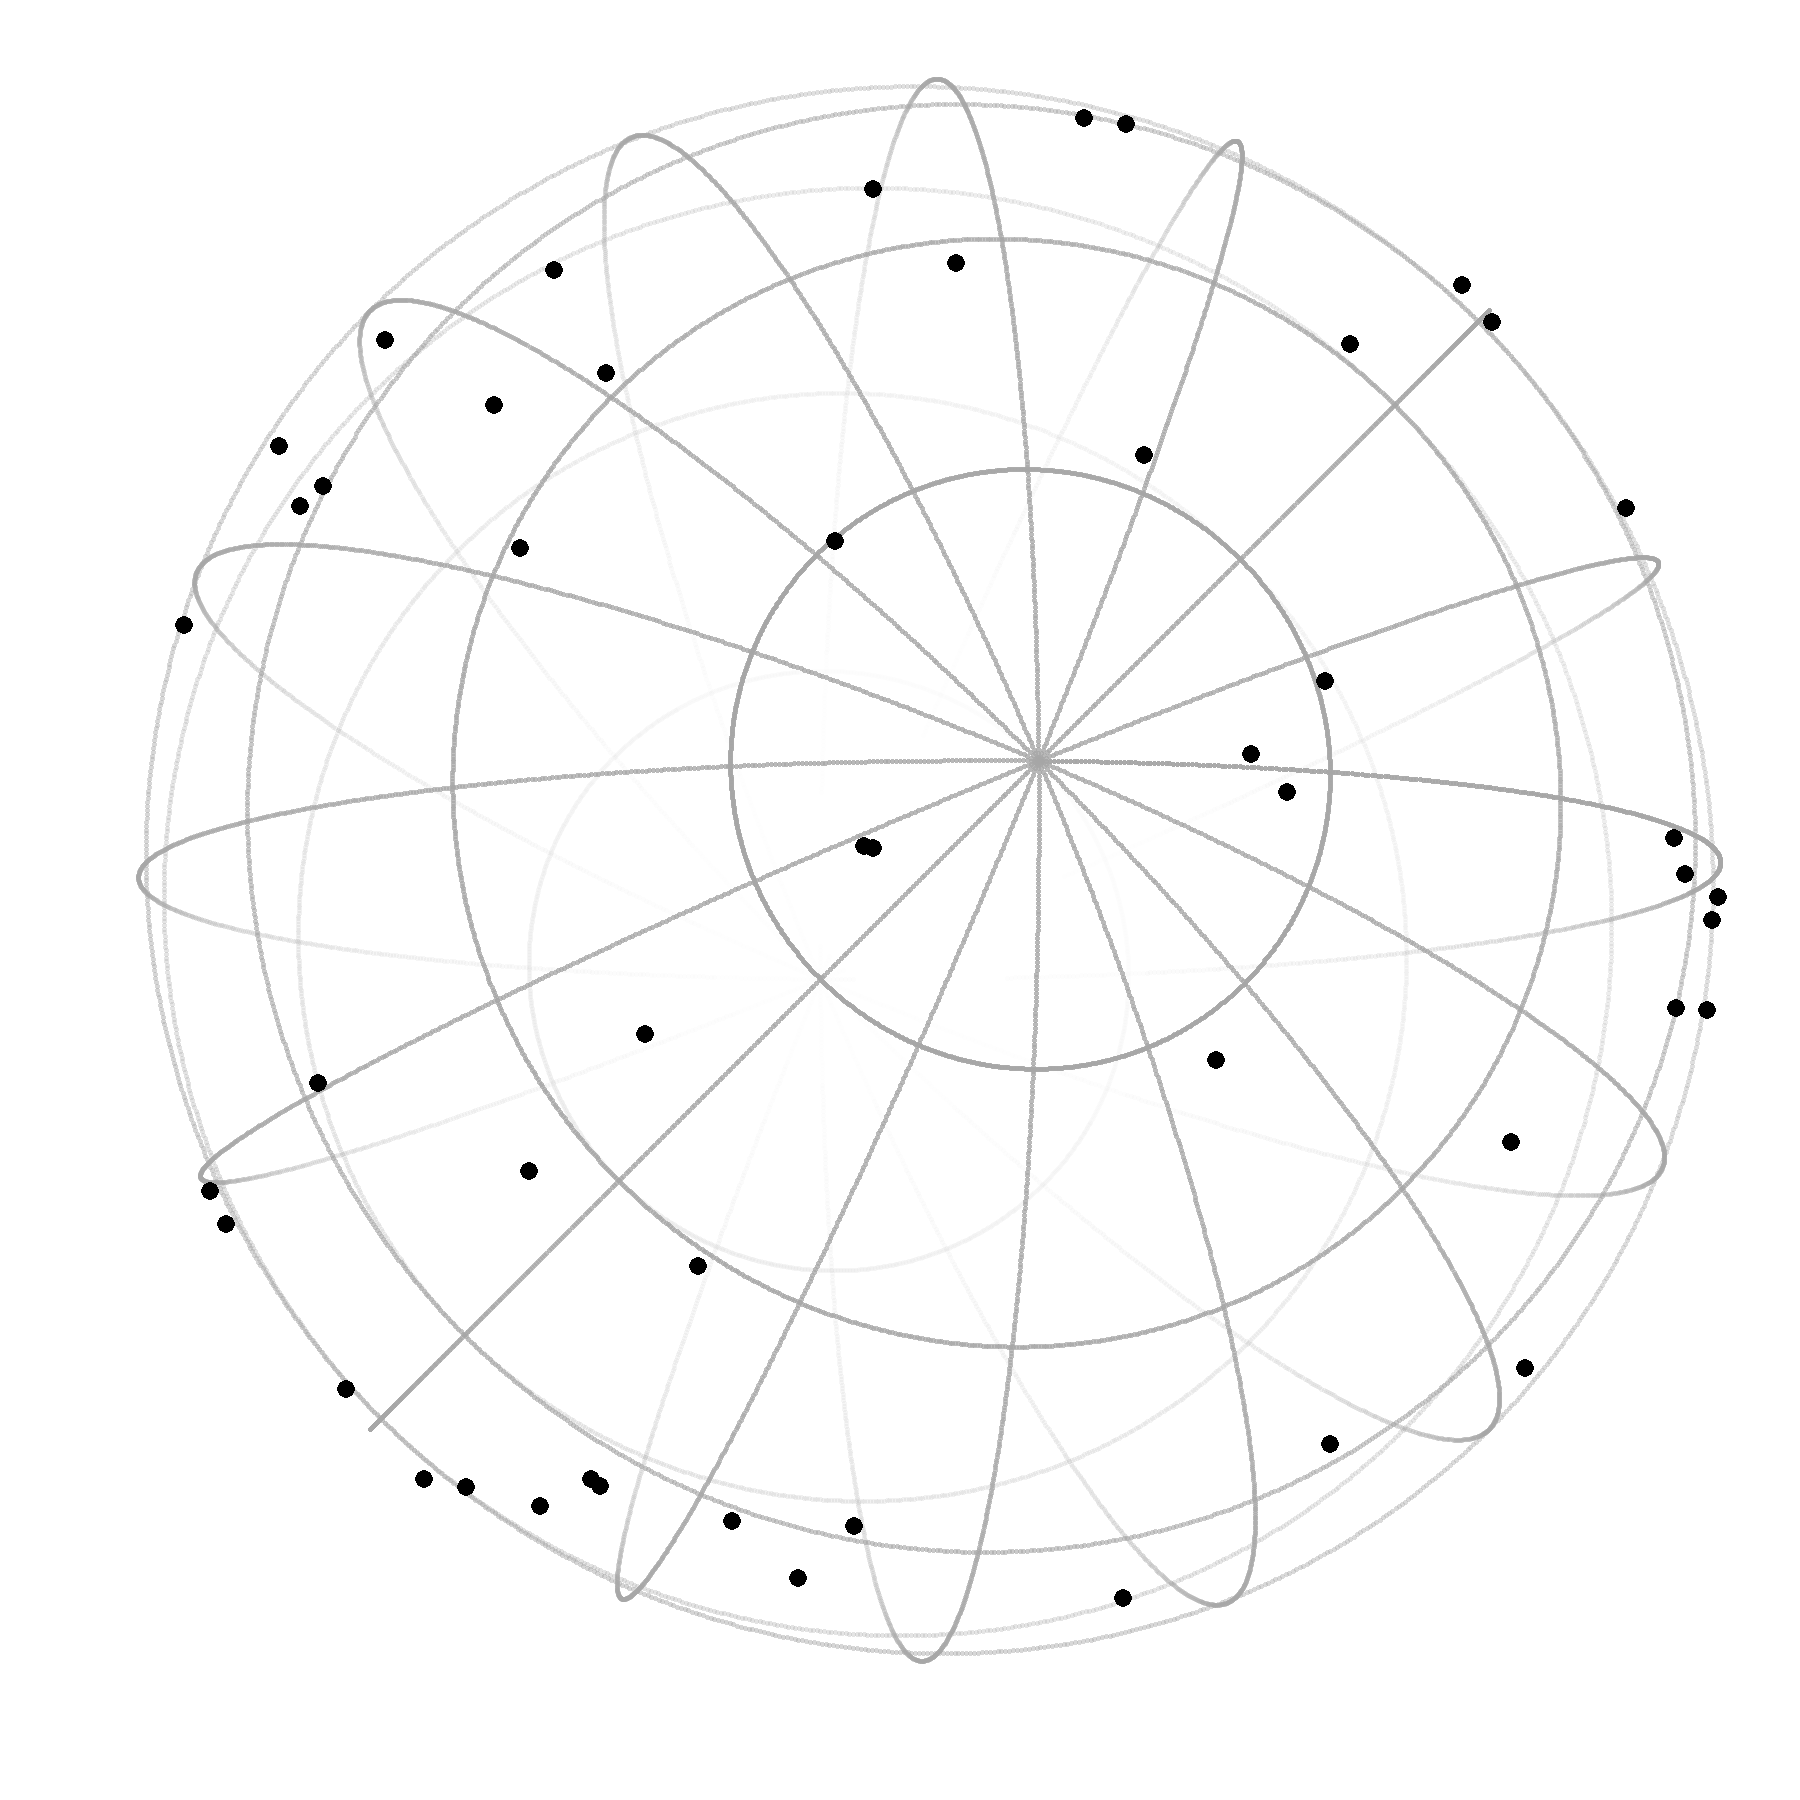
\includegraphics[width=\textwidth]{figures/eye1}
%		\caption{A random sample from the Cayley-UARS distribution with $\kappa=1$, $n=50$.}
%		\label{fig:sample}
%	\end{subfigure}
	\begin{subfigure}[h]{.45\textwidth}
		%\centering
		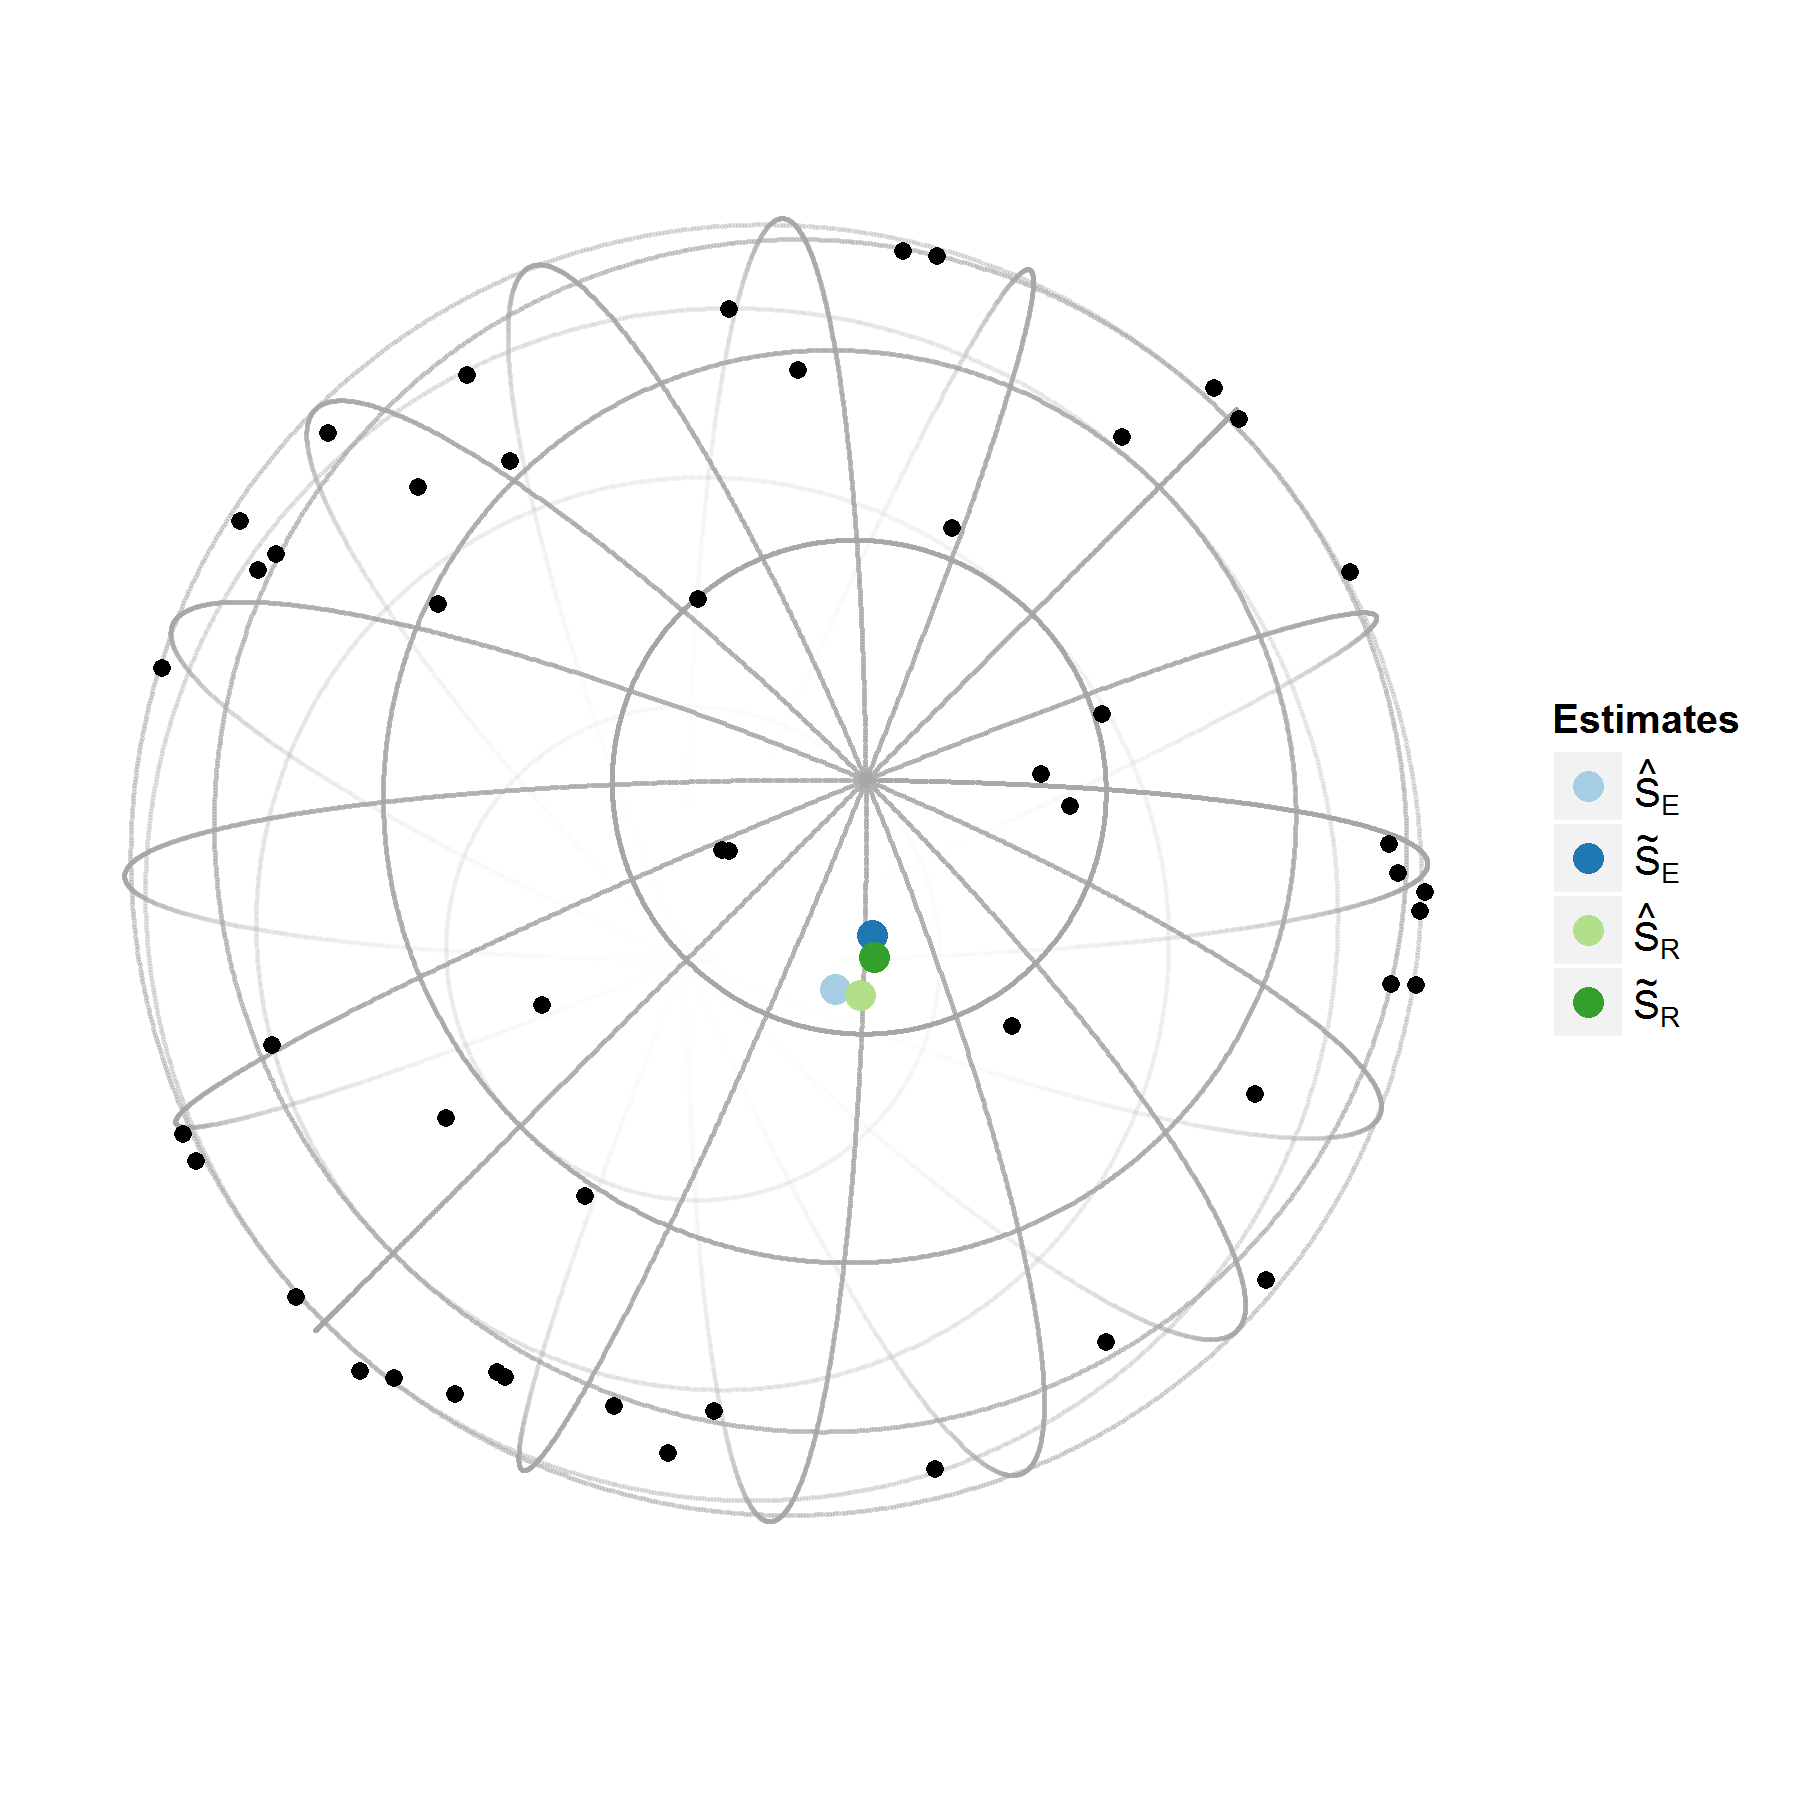
\includegraphics[width=\textwidth]{figures/eye2}
		\caption{All four of the estimators are plotted along with the random sample.}
		\label{fig:ests}
	\end{subfigure}
	\begin{subfigure}[h]{.45\textwidth}
		%\centering
		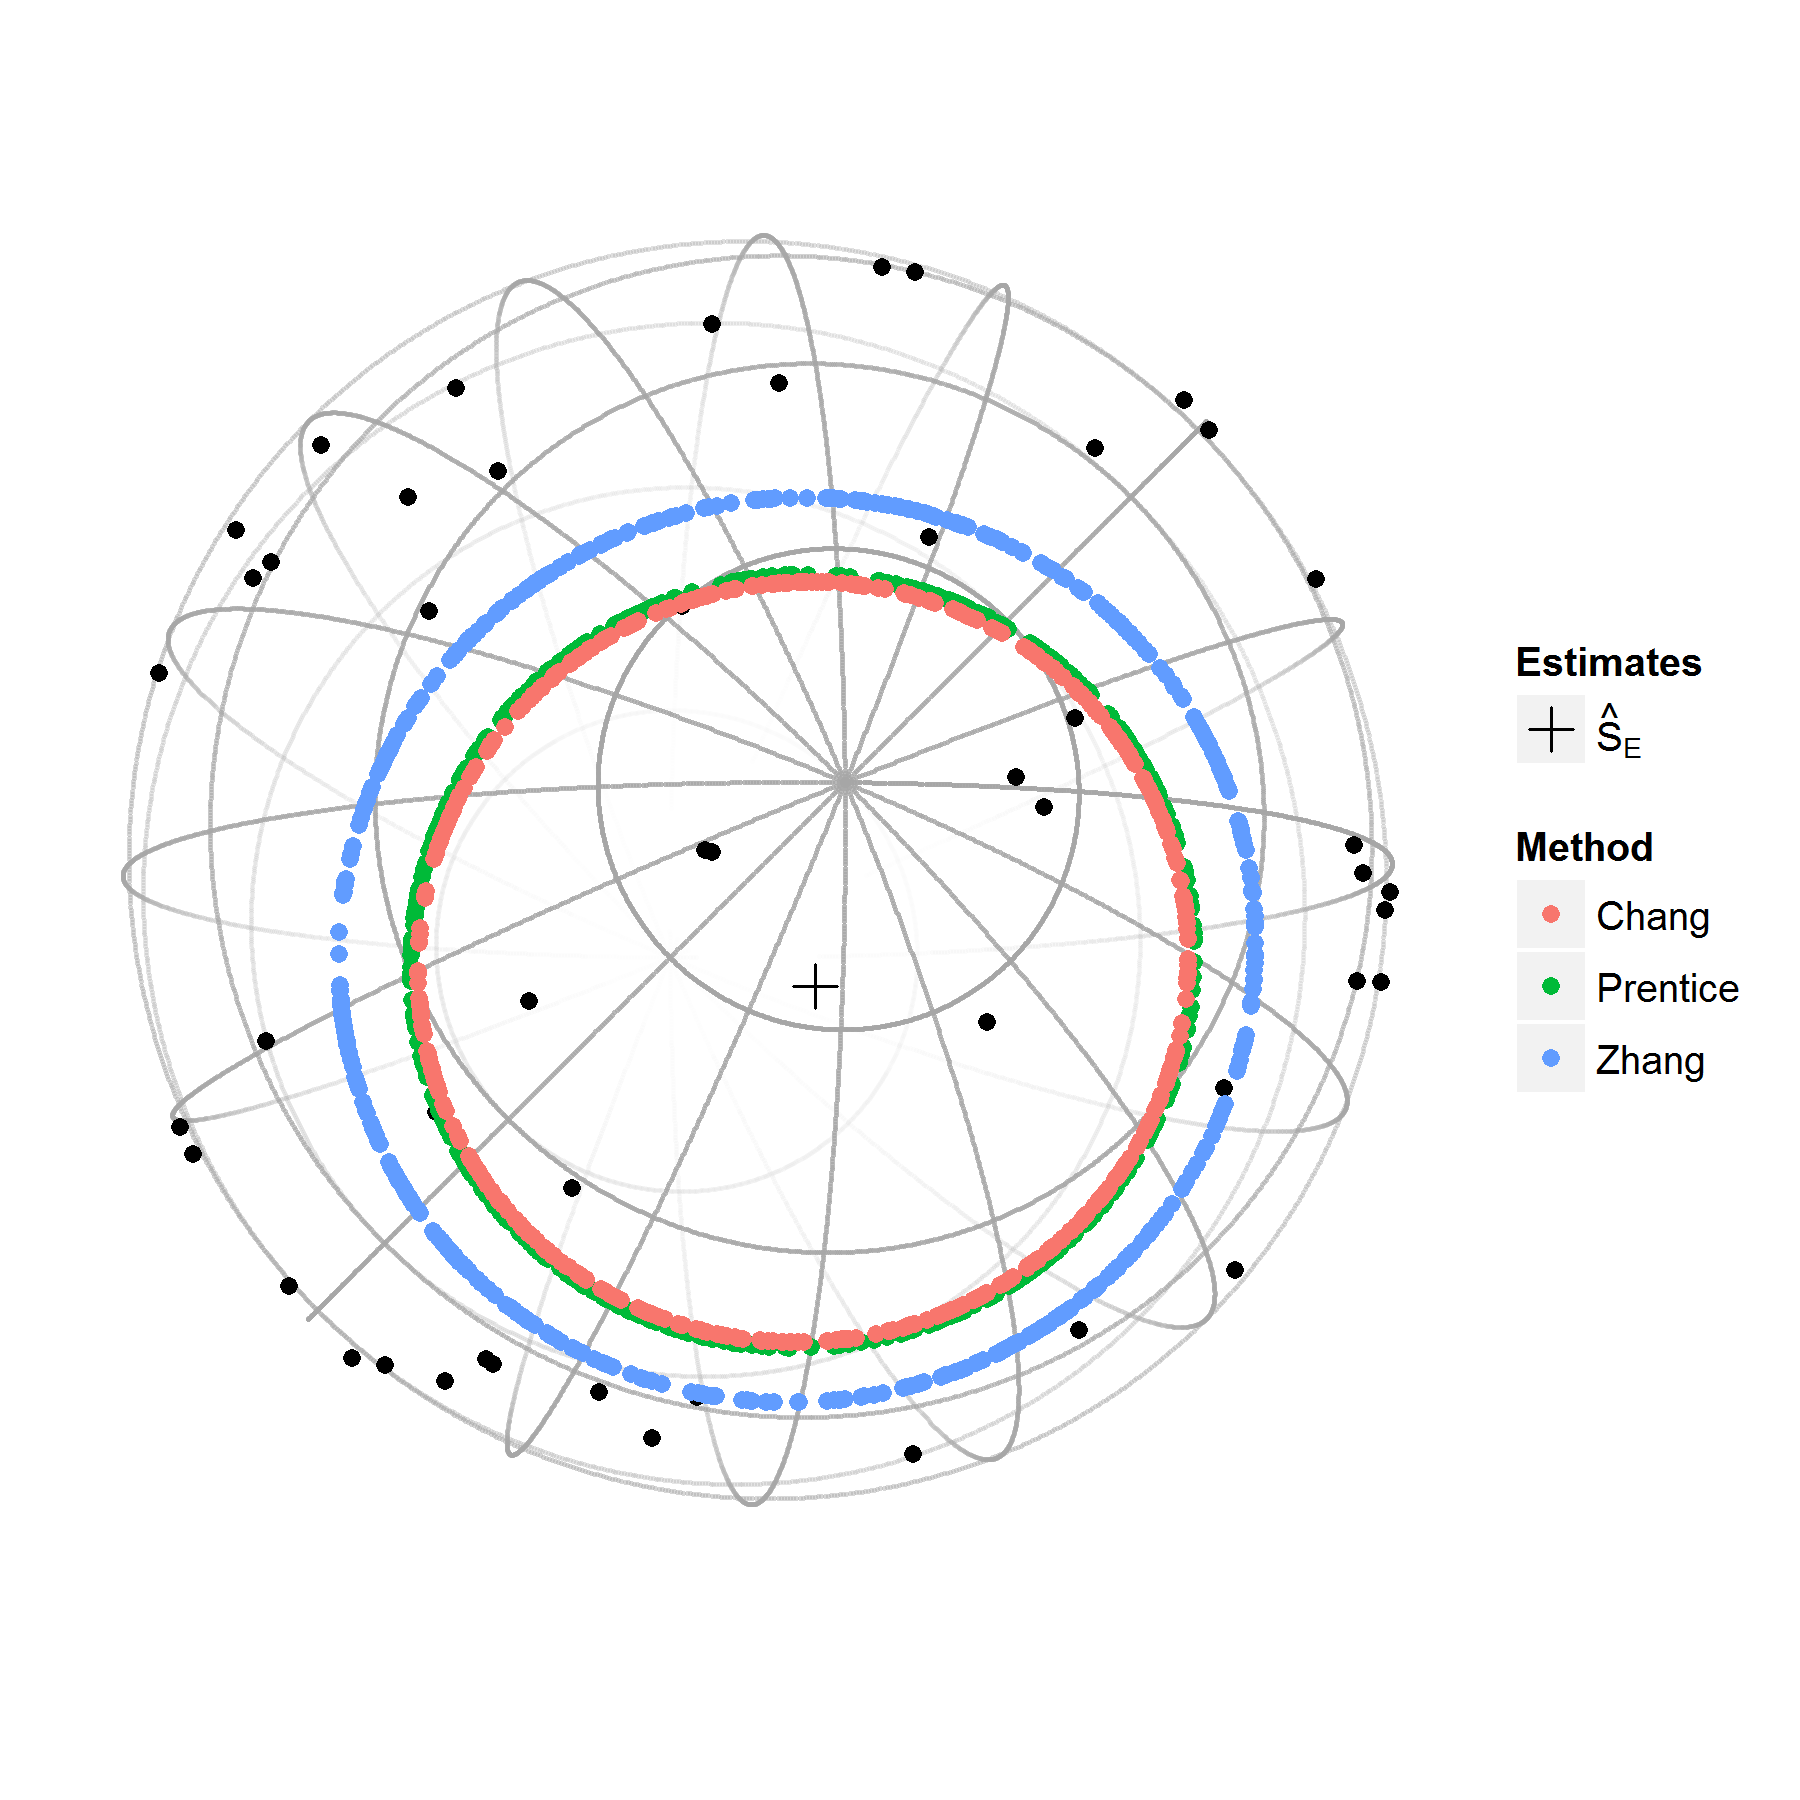
\includegraphics[width=\textwidth]{figures/eye3}
		\caption{Three methods to compute confidence regions for the projected mean.}
		\label{fig:regs}
	\end{subfigure}
	
	\caption{\label{figure:eye1}The $x$-axis of a random sample from the Cayley-UARS distribution with $\kappa=1$, $n=50$.}
	
\end{figure}

In Figure \ref{figure:eye1} a random sample of 50 matrices following the Cayley-UARS distribution with $\kappa=1$ is plotted along with four estimates of the central orientation.  The code to produce this plot is also given.

\section{Summary}

The \pkg{rotations} package is introduced and allows the user to create, simulate, analyze and visualize rotation data.  There are three parameterizations possible in this package and four built-in distributions from which data can be simulated.  The four estimators discussed in Stanfill et al. (2012) are each implemented and each can be visualized via \CRANpkg{ggplot2}.


\bibliography{stanfill-hofmann-genschel}

\address{Bryan Stanfill\\
  Department of Statistics\\
  Iowa State University\\
  Ames, IA 50011}\\
\email{stanfill@iastate.edu}

\address{Heike Hofmann\\
  Department of Statistics\\
  Iowa State University\\
  Ames, IA 50011}\\
\email{hofmann@mail.iastate.edu}

\address{Ulrike Genschel\\
  Department of Statistics\\
  Iowa State University\\
  Ames, IA 50011}\\
\email{ulrike@mail.iastate.edu}